%        File: WeeklyResearchReport_4_19_21.tex
%     Created: Mon Apr 19 08:00 AM 2021 E
% Last Change: Mon Apr 19 08:00 AM 2021 E
%
\documentclass[a4paper]{article}
\usepackage{mathtools}
\usepackage{verbatim}
\usepackage{graphicx}
\usepackage{tabularx}
\usepackage{pgfplots}
\usepackage{adjustbox}
\usepackage{booktabs}
\makeatletter
\let\latex@xfloat=\@xfloat
\def\@xfloat #1[#2]{%
    \latex@xfloat #1[#2]%
    \def\baselinestretch{1}
    \@normalsize\normalsize
    \normalsize
}
\makeatother
\usepackage{amsmath}
\usepackage{mathtools}
\usepackage{epigraph}
\usepackage{cancel}
\usepackage{xcolor}
\newcommand\Ccancel[2][black]{\renewcommand\CancelColor{\color{#1}}\cancel{#2}}
\usepackage{algorithm}
\usepackage{graphicx}
\usepackage[noend]{algpseudocode}
\usepackage{gnuplot-lua-tikz}
\usepackage[utf8]{inputenc}
\usepackage{pgfplots}
\usepackage{tabularx}
\DeclareUnicodeCharacter{2212}{−}
\usepgfplotslibrary{groupplots,dateplot}
\usetikzlibrary{patterns,shapes.arrows}
\pgfplotsset{compat=newest}
\begin{document}
\begin{titlepage}

    \title{
    Daily Research Report}

    \author{ Jeffrey Severino \\
        University of Toledo \\
        Toledo, OH  43606 \\
    email: jseveri@rockets.utoledo.edu}


    \maketitle

\end{titlepage}
% \section{Introduction}
% \begin{enumerate}
%     \item Get the reader\'s attention
%     \item Summary of previous research - what is already known about the topic
%     \item Set up research by formulating a clear problem to be solved - what
%         is not known yet.
%     \item Propose a hypothesis to test
%     \item State the main purpose
% \end{enumerate}
% Hypothesis: Increasing the number of grid points will 
\section{Current Research Direction}
Finalized the post processing method for the code validation.
\section{Research Performed}

\begin{itemize}
    \item Fixed the post processing code to take the indicies of the axial wavenumber as an
input. 
\item Ran the same cases for fourth order differencing. If there is an index conflict, it
    will be easy to change.
\item Explored various ways of plotting propagating and decaying modes. I think
    I should limit the number of modes per plot to two. 
\end{itemize}


\section{Issues and Concerns}
Running the fourth order scheme gives me a SIGFPE error that needs investigation. 
Where is it coming from and is this where I absolutely need dissipation? I 
have not added any and I definitely need to start running smoothing coefficients
to see how much is needed. Interestingly enough, there is no literature on
how much to use.

The plots are way too crowded now, I need a checklist for the plots that I want to
show to start building the table of figures.


 \begin{figure}
     \centering
     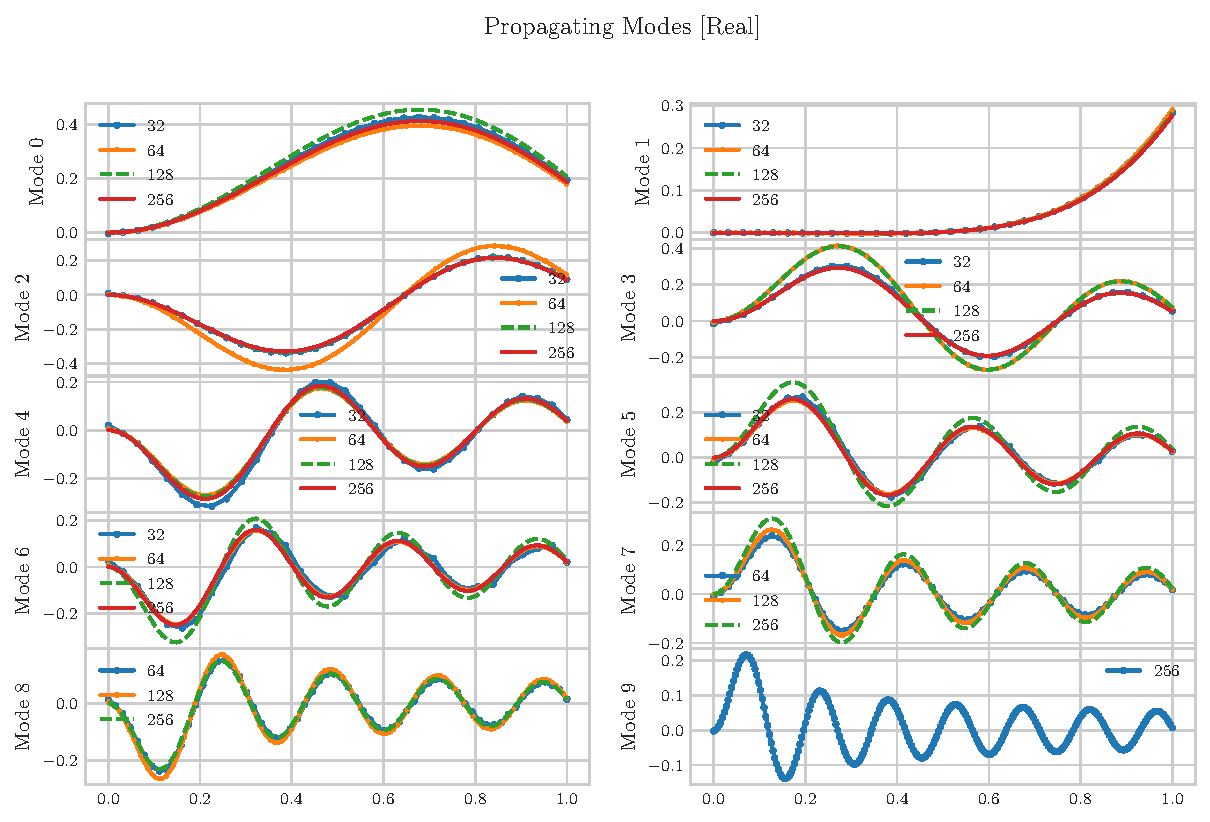
\includegraphics[width=\textwidth]{/home/jeff-severino/SWIRL/CodeRun/03-plotReport/tex-outputs/egv_prop_re.pdf}
 \end{figure}


 \begin{figure}
     \centering
     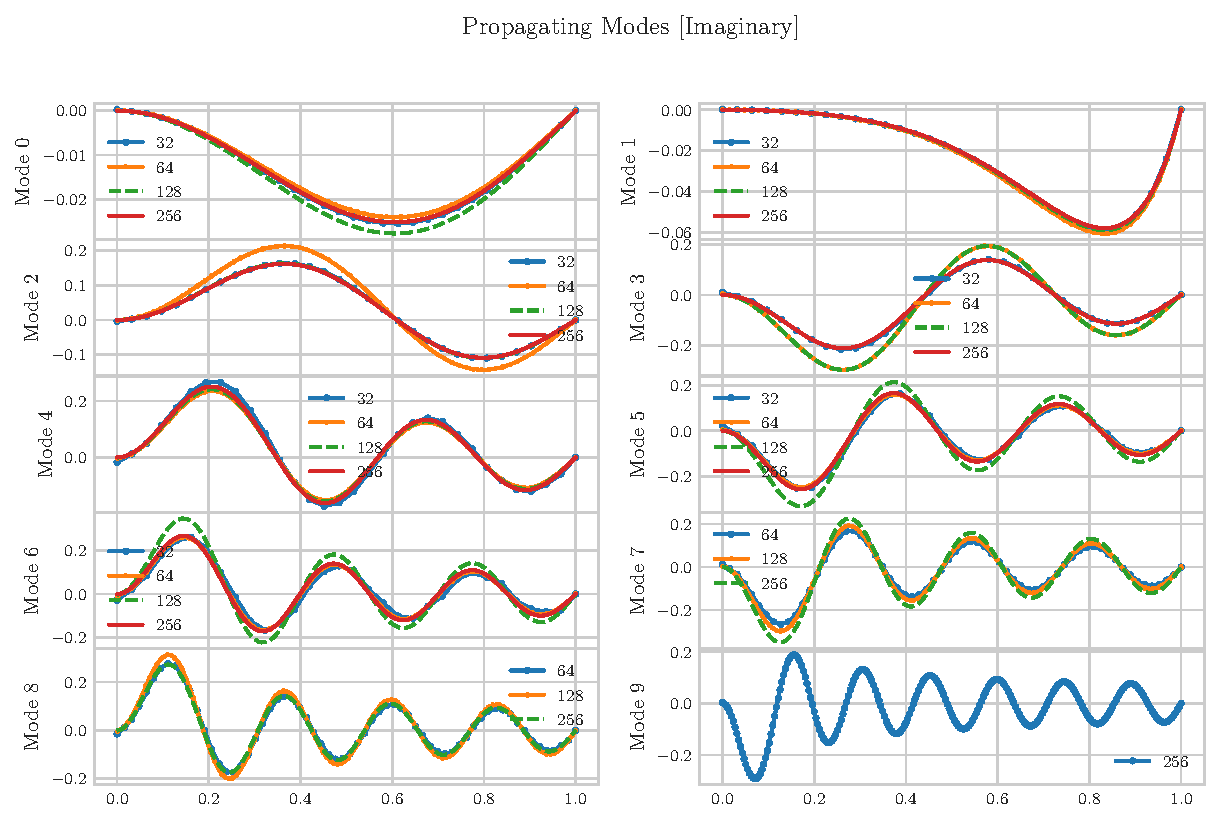
\includegraphics[width=\textwidth]{/home/jeff-severino/SWIRL/CodeRun/03-plotReport/tex-outputs/egv_prop_im.pdf}
 \end{figure}


 \begin{figure}
     \centering
     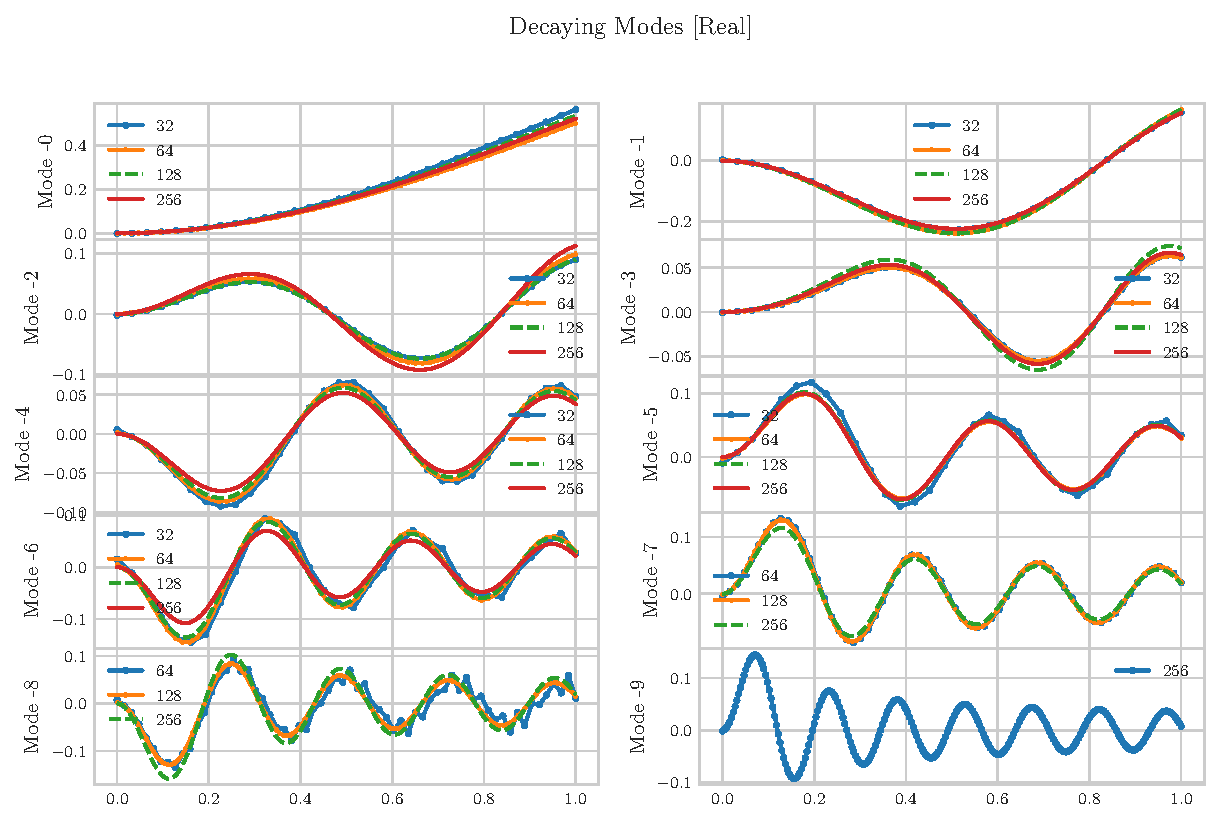
\includegraphics[width=\textwidth]{/home/jeff-severino/SWIRL/CodeRun/03-plotReport/tex-outputs/egv_decay_re.pdf}
 \end{figure}


 \begin{figure}
     \centering
     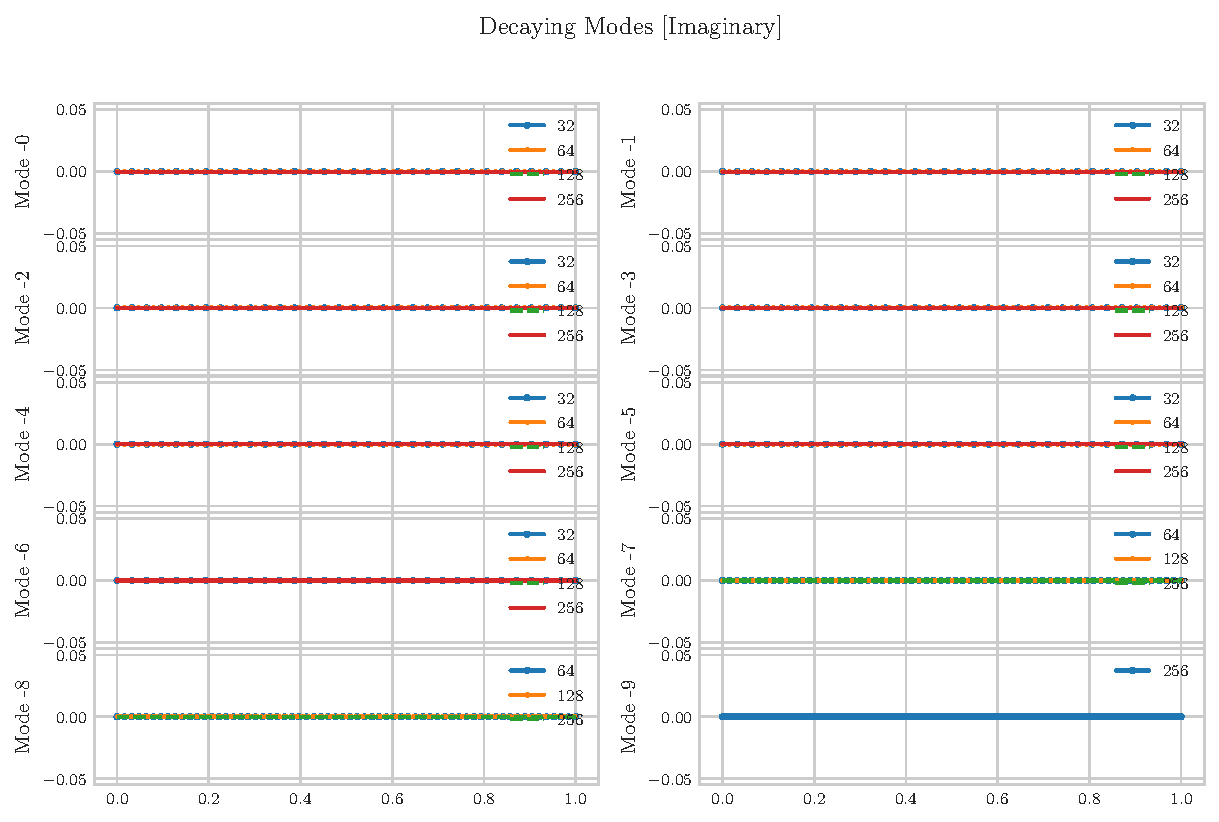
\includegraphics[width=\textwidth]{/home/jeff-severino/SWIRL/CodeRun/03-plotReport/tex-outputs/egv_decay_im.pdf}
 \end{figure}



\section{Planned Research}

Plot the axial wavenumbers for the two schemes (2nd and 4th) with and without
dissipation. There are modes that do not correspond to the modes reported in 
Shankar and Kousen. Are these modes physical? i.e. What happens to them as 
I add dissipation instead of higher number of grid points? What if I do both?


\end{document}


